\section{Definitions}
This section covers and differentiates between the basic non-mathematical definitions and terms used in this thesis.

\subsection{Virtual and augmented reality}\label{sec:VAR}
The words virtual reality (VR) and augmented reality (AR) can be constantly read in the recent news all over the internet and other media. However, they are used in various contexts and are often defined differently. The definition used in this thesis is therefore only one small aspect of the whole field and should help to differentiate between the two concepts. 
\subsubsection{Virtual reality}
Virtual reality\index{Virtual reality} can be defined as \enquote{an electronic simulation in which images are generated in real time (...) from a stored database and displayed in such a way as to facilitate real-time interaction with the database (...).} \cite[p.148]{Latham.1995}

A virtual reality application uses a combination of software and hardware to let the user experience immersion, interaction and imagination (the three I's of virtual reality) in a virtual world. Whereas the first two I's should be clear and understandable, the last one is often underrated or even left out. Since virtual reality only counts on virtual content and given the fact that computer graphics are still not a perfect representation of our \enquote{reality}, the user's imagination is a very important aspect of an application (\cite[p.3 et seq.]{Burdea.2003}).

Typically, a common computer game can not be classified as a virtual reality application unless it includes the collection and usage of other data than only the keyboard and mouse inputs. For this purpose, a VR application often comes with other interfaces such as a head-mounted display (HMD)\index{Head-mounted display} \footnote{The idea of a HMD started with Morton Heilig's  \index{Morton L. Heilig} U.S. patent in 1960 (see \cite{Heilig.1957}). Recent popular models include the \textit{Oculus Rift} (see \cite{Oculus.2016})\index{Head-mounted display!Oculus Rift} and \textit{Google Cardboard} (see \cite{GoogleDev.2016})\index{Head-mounted display!Google Cardboard}. The HMD tracks, amongst other things, the head position and its movement and displays the stereo image.}. An imaginary example for a perfect virtual reality environment is Star Trek's Holodeck, as mentioned before (\autoref{sec:preface}).

\subsubsection{Augmented reality}
\begin{figure}[htbp]
		\centering
		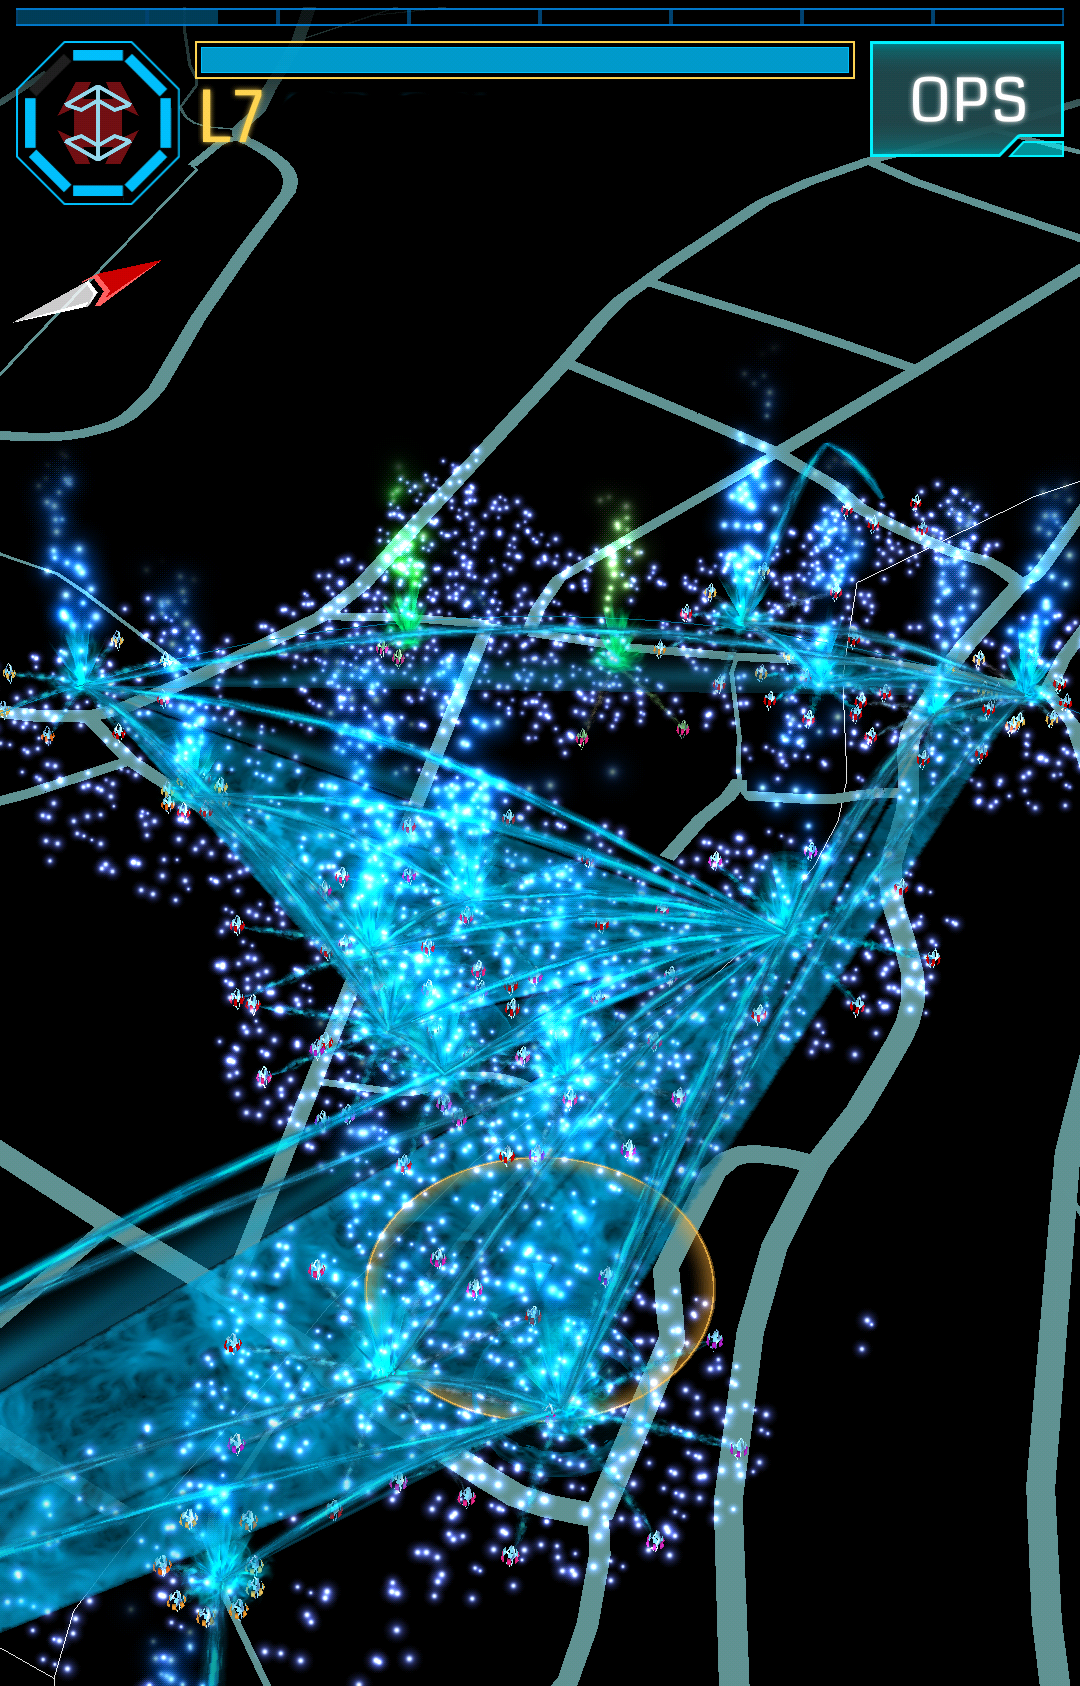
\includegraphics[width=0.4\textwidth]{figures/Ingress}
		\caption[Screenshot of the mobile AR game Ingress]{Screenshot of the mobile AR game Ingress showing the portals around the Hochschule Furtwangen University (\textit{source:} \cite{Haefele.2014}).}
		\label{fig:Ingress}
\end{figure}
In comparison to virtual reality, augmented reality \index{Augmented reality} extends our \enquote{real world} with virtual (digital) content, which must be embedded seamlessly to provide a fully immersive experience. The users can interact with virtual objects and can be provided with relevant additional information about their environment. The virtual data is computed in real-time and is displayed as an overlay on top of the \enquote{real world} in front of the user's eyes. AR highly relies on its technologies. Relevant topics, amongst others, are object recognition, location tracking, interfaces\footnote{A common interface for AR was and still is the head-up display (HUD)\index{Head-up display}, often used for military application (see \cite[p.6]{Burdea.2003}). But also immaterial displays, such as fog screens, are researched (see \cite[p.25 et seq.]{Toennis.2010}).} and real-time computation (compare with \cite[p.1 et seqq.]{Toennis.2010}). 

The game \textit{Ingress}\index{Ingress} by \textit{Niantic, Inc.} (see \autoref{fig:Ingress} for a screenshot), in which two factions fight over virtual portals, is an example for a location-based mobile AR game. The portals, which are linked to real places all over the world, and other game functions are displayed on the user's mobile device in real-time. The users travel to these real places to conquer or defend the portals in the name of their faction (\cite{Niantic.2016}). 

\subsection{Computer vision}\label{ssec:cv}
Computer vision\index{Computer vision} (also often referred to as \enquote{machine vision}) is the \enquote{automated extraction of information from images} (\cite{Lowe.2016}). It also refers to a whole science field, which combines several disciplines\footnote{That among are mathematics and computer science, as well as phsyics, the psychology of perception and the neuro sciences (\cite[p.xi]{Hartley.2011}).} to research how to make a computer see. The word is differentiated from the wide field of image processing, in which images are processed in different ways to produce new images (compare with \cite{Lowe.2016}).
 
As already stated in the preface, the visual modeling of perception was underestimated by scientists of the Artificial Intelligence for a long time. Although it is still not clear whether computer vision should be created on the bases of biological patterns, understanding how biological vision in general and human depth perception in particular work seems to be a necessity\footnote{Attempts to find new approaches have  not been successful yet.} (compare with \textit{Oliver Faugeras'} foreword in \cite[p.xi]{Hartley.2011}). For this a short overview shall be given in \autoref{ssec:hv}.  

\todo{multiple view geometry? stereo vision? --> algorithms examples: structure from motion, stereo matching --> see math. principles!}
\index{Stereo vision}
 
\subsection{Human depth perception}\label{ssec:hv}
First of all, our three-dimensional perception is actually based on a two-dimensional image which is projected on our retina. But out of these 2-D images we still get information about how far away an object is. These information are called \textit{depth cues}\index{Depth cues}, whose connection to the actual depth of field we learn from experience (\cite[p.28]{Hottong.2009}). 

The depth cues can be classified into three different groups (freely adapted from \cite{Goldstein.2015} and \cite[p.28 et seqq.]{Hottong.2009} \todo{page 186?}):
\begin{description}
\item [Oculomotor depth cues\index{Depth cues!Oculomotor depth cues}]\hfill \\ These cues provide depth information for objects which are in closer range (one meter or below). Our brain receives and analyzes feedback from the eye muscles which are contracted differently depending on the distance of the object which gets focused on. The oculomotor cues are based on two factors: \textit{accommodation}\index{Depth cues!Accommodation} and \textit{convergence}\index{Depth cues!Convergence}\footnote{The first is based on the contraction of the ciliary muscles, which let the eye lens take on different shapes. The latter uses the information of the eyes' convergence movements during their fixation on a moving object to estimate distances.}.
\item [Monocular depth cues\index{Depth cues!Monocular depth cues}]\hfill \\
\item [Binocular or stereoscopic depth cues\index{Depth cues!Binocular depth cues}]\hfill \\
\end{description} 
  
\todo{get real book}\\


